%
% dilatation.tex -- template for standalon tikz images
%
% (c) 2019 Prof Dr Andreas Müller, Hochschule Rapperswil
%
\documentclass[tikz]{standalone}
\usepackage{amsmath}
\usepackage{times}
\usepackage{txfonts}
\usepackage{pgfplots}
\usepackage{csvsimple}
\usetikzlibrary{arrows,intersections,math}
\begin{document}
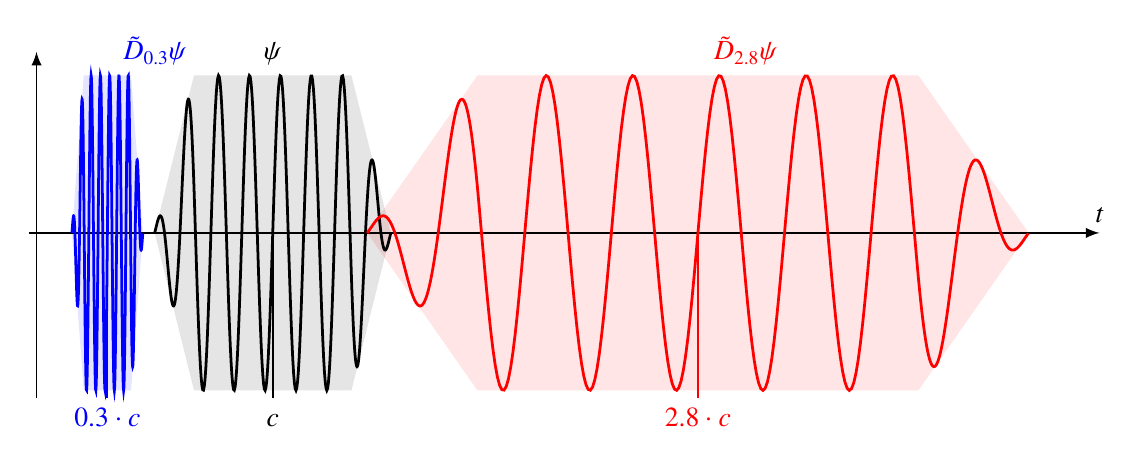
\begin{tikzpicture}[>=latex]

\def\pivalue{3.14159}

\def\bone{2.8}
\def\btwo{0.3}
\def\frequency{16}

\fill[color=gray!20] (1.5,0)--(2,-2)--(4,-2)
	--(4.5,0)--(4,2)--(2,2)--cycle;

\fill[color=blue!10] ({1.5*\btwo},0)--({2*\btwo},-2)--({4*\btwo},-2)
	--({4.5*\btwo},0)--({4*\btwo},2)--({2*\btwo},2)--cycle;
\fill[color=red!10] ({1.5*\bone},0)--({2*\bone},-2)--({4*\bone},-2)
	--({4.5*\bone},0)--({4*\bone},2)--({2*\bone},2)--cycle;

\begin{scope}
\clip (1.5,0)--(2,-2)--(4,-2)--(4.5,0)--(4,2)--(2,2)--cycle;
\definecolor{bluegray}{rgb}{0.8,0.8,0.9}
\definecolor{redgray}{rgb}{0.9,0.8,0.8}
\fill[color=bluegray] ({1.5*\btwo},0)--({2*\btwo},-2)--({4*\btwo},-2)
	--({4.5*\btwo},0)--({4*\btwo},2)--({2*\btwo},2)--cycle;
\fill[color=redgray] ({1.5*\bone},0)--({2*\bone},-2)--({4*\bone},-2)
	--({4.5*\bone},0)--({4*\bone},2)--({2*\bone},2)--cycle;
\end{scope}

\draw[->,line width=0.7pt] (-0.1,0)--(13.5,0) coordinate[label={$t$}];
\draw[->,line width=0.7pt] (0,-2.1)--(0,2.3);

%\foreach \x in {1,...,13}{
%	\draw[line width=0.7pt] ({\x},-0.1)--({\x},0.1);
%}

\node at (3,2) [above] {$\psi$};
\node[color=blue] at (1.5,2) [above] {$\tilde{D}_{\btwo}\psi$};
\node[color=red] at (9,2) [above] {$\tilde{D}_{\bone}\psi$};

\draw[line width=1pt]
	plot[domain=-1.5:-1,samples=100]
		({\x+3},{2*2*(\x+1.5)*sin(\frequency*\x*(180/\pivalue))}) --
	plot[domain=-1:1,samples=200]
		({\x+3},{2*sin(\frequency*\x*(180/\pivalue))}) --
	plot[domain=1:1.5,samples=100]
		({\x+3},{-2*2*(\x-1.5)*sin(\frequency*\x*(180/\pivalue))});

\draw[color=blue,line width=1pt]
	plot[domain=-1.5:-1,samples=100]
		({(\x+3)*\btwo},{2*2*(\x+1.5)*sin(\frequency*\x*(180/\pivalue))}) --
	plot[domain=-1:1,samples=200]
		({(\x+3)*\btwo},{2*sin(\frequency*\x*(180/\pivalue))}) --
	plot[domain=1:1.5,samples=100]
		({(\x+3)*\btwo},{-2*2*(\x-1.5)*sin(\frequency*\x*(180/\pivalue))});

\draw[color=red,line width=1pt]
	plot[domain=-1.5:-1,samples=100]
		({(\x+3)*\bone},{2*2*(\x+1.5)*sin(\frequency*\x*(180/\pivalue))}) --
	plot[domain=-1:1,samples=200]
		({(\x+3)*\bone},{2*sin(\frequency*\x*(180/\pivalue))}) --
	plot[domain=1:1.5,samples=100]
		({(\x+3)*\bone},{-2*2*(\x-1.5)*sin(\frequency*\x*(180/\pivalue))});

\draw[color=red,line width=0.7pt] ({3*\bone},0)--({3*\bone},-2.1);
\node[color=red] at ({3*\bone},-2.1) [below] {$\bone\cdot c\mathstrut$};
\draw[color=blue,line width=0.7pt] ({3*\btwo},0)--({3*\btwo},-2.1);
\node[color=blue] at ({3*\btwo},-2.1) [below] {$\btwo\cdot c\mathstrut$};
\draw[line width=0.7pt] (3,0)--(3,-2.1);
\node at (3,-2.1) [below] {$c\mathstrut$};

\end{tikzpicture}
\end{document}

